\documentclass[numberedappendix]{aastex6}

\usepackage{graphicx}

\usepackage{hyperref}

\newcommand{\maestro}{{\sffamily Maestro}}
\newcommand{\castro}{{\sffamily Castro}}
\newcommand{\starkiller}{{\sffamily StarKiller}}
\newcommand{\starlord}{{\sffamily StarLord}}
\newcommand{\nyx}{{\sffamily Nyx}}
\newcommand{\amrex}{{\sffamily AMReX}}


\usepackage{color}
\setlength{\marginparwidth}{0.75in}
\newcommand{\MarginPar}[1]{\marginpar{\vskip-\baselineskip\raggedright\tiny\sffamily\hrule\smallskip{\color{red}#1}\par\smallskip\hrule}}



\begin{document}

\title{Preparing an AMR Library for Summit}
\shortauthors{Katz et al.}

\author{Max Katz\altaffilmark{1,2}}
\author{Maria Barrios Sazo\altaffilmark{2}}
\author{Brian Friesen\altaffilmark{3}}
\author{Adam Jacobs\altaffilmark{4}}
\author{Xinsheng Qin\altaffilmark{5}}
\author{Donald Willcox\altaffilmark{2}}
\author{Michael Zingale\altaffilmark{2}}

\altaffiltext{1}
{
  NVIDIA Corporation
}

\altaffiltext{2}
{
  Department of Physics and Astronomy, Stony Brook University
}

\altaffiltext{3}
{
  National Energy Research Scientific Computing Center, Lawrence Berkeley National Laboratory
}

\altaffiltext{4}
{
  Department of Physics and Astronomy, Michigan State University
}

\altaffiltext{5}
{
  Department of Civil and Environmental Engineering, University of Washington
}

\begin{abstract}
  This document contains the session description and extended abstract for
  a submission to GTC 2018.
\end{abstract}

\section{Session Description}

In this session you'll hear about one team's experience preparing an adaptive mesh
refinement library -- and a fluid dynamics code based on it -- for Summit, the
IBM POWER9 and NVIDIA Volta system at Oak Ridge National Laboratory, where multiple GPUs
are connected via NVLink to each other and the CPUs. It was simple to compile and run on
the OpenPOWER architecture, and to offload to the GPUs with CUDA Fortran, with little
architecture-specific code. Initial results with POWER8 and P100 have shown 
excellent CPU and GPU performance and good multi-node scaling for an astrophysics mini-app
that was difficult to run effectively on prior GPU architectures. We will also discuss
our experiences porting other modules in our multi-physics codes, and preliminary
results on the POWER9 and V100 platform.

\section{Extended Abstract}

AMReX (Adaptive Mesh Refinement for Exascale) is a software library funded by an
Exascale Computing Project Co-Design Center, with the goal of preparing for the upcoming
generations of US Department of Energy supercomputers. One aspect of this is an initial
exploration of heterogeneous CPU and GPU systems, including the Summit system at Oak Ridge
National Laboratory, which will come online in 2018. One of the key science areas supported
by AMReX is multi-scale, multi-physics codes, where a hydrodynamics module is combined with
other physics such as radiation, gravity, chemical or nuclear reactions, or electromagnetic
fields, to do simulation in a wide range of fields, ranging from cosmology to particle accelerators.
AMReX has been extensively optimized for traditional CPU performance, including
the Intel MIC architecture \citep{boxlib-tiling}. The team's efforts
on GPUs are more recent. Initial evaluation began several years ago with OpenACC
by our team's collaborators in astrophysics, using the code CASTRO \citep{castro}. Recently we
restarted from scratch using Unified Memory for Pascal as the basis for data management,
and CUDA Fortran for offloading compute onto the GPUs, in such a way that the individual
physics codes built on top of AMReX would have to apply minimal refactoring to their
software to get code working on the GPU.

To test this strategy, we stripped down CASTRO to a mini-app containing just the
hydrodynamics module, and prepared it to run on the IBM Minsky nodes on Summitdev
at Oak Ridge (20 POWER8 CPU cores and 4 P100 GPUs connected via NVLink). Like other
hydrodynamics benchmarks, we evaluated performance on the classic Sedov-Taylor blast
wave problem, using a Figure of Merit (FoM) measuring the number of zones advanced
per microsecond. The FoM is typically 0.01 to 0.05 for a single CPU core. Using all 20 CPU cores and
4 hardware threads each, we obtained a peak FoM of 0.9 (compare to a peak FoM
of 0.75 on a single Knight's Landing node using 68 cores and 4 hardware threads).
For a single P100 GPU, the peak FoM is 2.4. We demonstrated scaling results using up to
32 nodes on Summitdev, with 128 GPUs, and observe 70-80\% efficiency relative to perfect
linear scaling. It should be noted that these results are preliminary, and that on all
architectures, we did very little optimization work, so this should not be construed
as a direct comparison between the architectures. However, it is an encouraging result,
as we were still able to obtain very good performance.

For comparison, the FoM on a single K20 GPU is two orders of magnitude smaller than for P100.
We have also run the same code on a single pre-production V100 (without any Volta or CUDA 9 optimization)
and found that the FoM is a factor of two larger than on P100. Prior to GTC, we will repeat
this measurement on production hardware, and experiment with multi-GPU and multi-node
behavior, to the extent that the systems at Oak Ridge and Livermore are ready for this.

\begin{figure}[h!]
  \begin{center}
    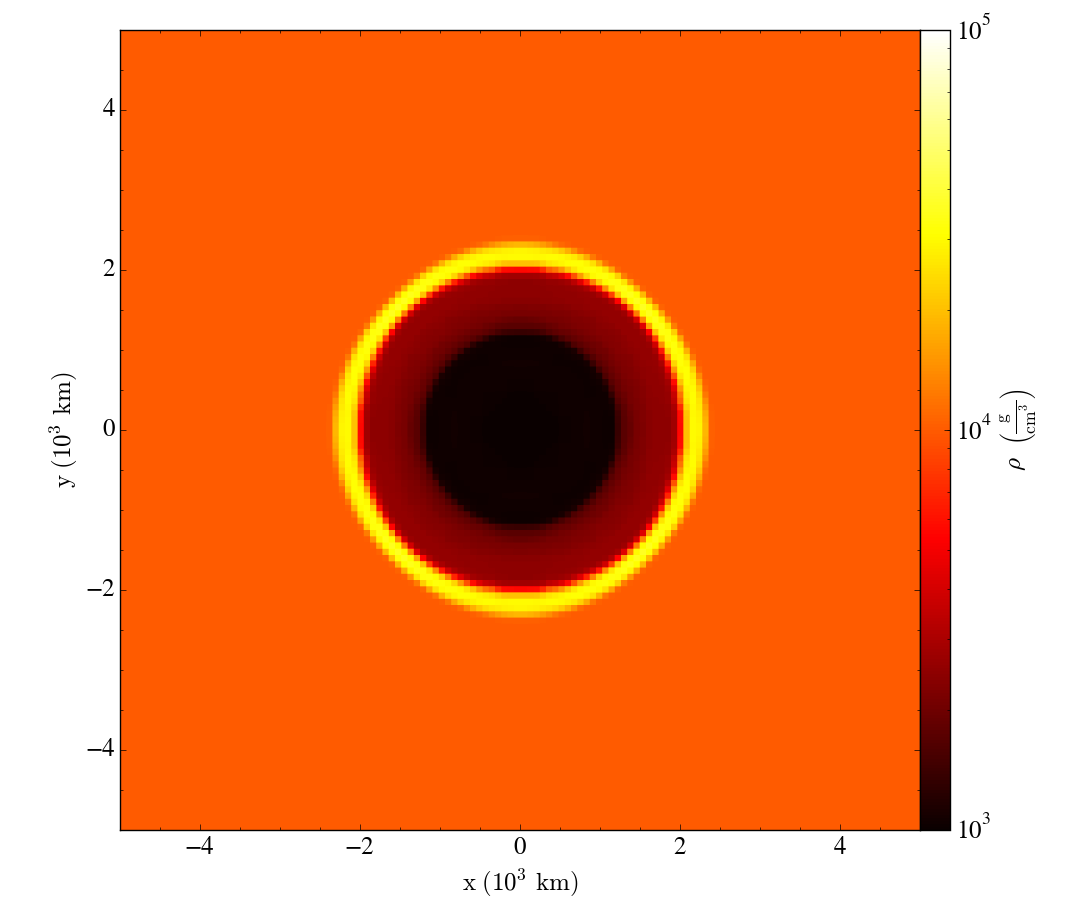
\includegraphics[scale=0.65]{sedov.png}
    \caption{A visualization of the Sedov-Taylor blast wave problem. A large amount of energy
      is deposited in a small region at the center of the domain, and this creates a shock
      wave that propagates outward in all directions. This image shows this spherical blast
      wave expanding outwards, in a 2D slice of the 3D simulation.}
  \end{center}
\end{figure}

\begin{figure}[h!]
  \begin{center}
    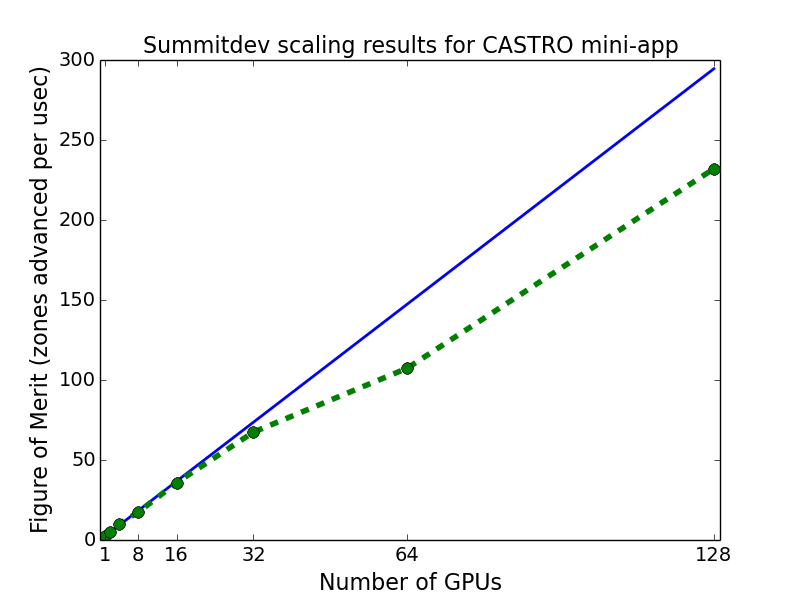
\includegraphics[scale=0.65]{scaling.png}
    \caption{Scaling of the Sedov-Taylor blast wave problem. This test was run
      on Summitdev at Oak Ridge, with 4 P100 GPUs per node. The domain was decomposed with
      a single MPI rank per GPU, and the problem size was scaled so that the portion
      of the domain owned by each GPU filled a substantial fraction of the 16 GB memory
      without oversubscribing it (so, on the single GPU test, 2 million zones were
      evolved, while on the 128 GPU test, 450 million zones total were evolved). The
      performance is measured in terms of the average number of zones advanced per
      microsecond. The data is marked by solid circles and is connected by a dashed
      line. A solid curve shows perfect linear weak scaling.}
  \end{center}
\end{figure}

\clearpage

\section{Acknowledgements}

The work at Stony Brook was supported by DOE/Office of Nuclear
Physics grant DE-FG02-87ER40317 and NSF award AST-1211563.  An award
of computer time was provided by the Innovative and Novel
Computational Impact on Theory and Experiment (INCITE) program.  This
research used resources of the Oak Ridge Leadership Computing Facility
at the Oak Ridge National Laboratory, which is supported by the Office
of Science of the U.S. Department of Energy under Contract
No.\ DE-AC05-00OR22725.  We appreciate the efforts of the OLCF (and in
particular Fernanda Foertter) in organizing GPU hackathons.  This
research used resources of the National Energy Research Scientific
Computing Center, which is supported by the Office of Science of the
U.S. Department of Energy under Contract No.\ DE-AC02-05CH11231.
Development work benefited from a grant of a Titan X Pascal GPU
from NVIDIA through the GPU Grant Program, as well as access to
the CORAL Early Access systems: Summitdev at ORNL, and ray and rzmanta
at LLNL.

\bibliographystyle{aasjournal}
\bibliography{refs}

\end{document}
